% !TeX root = holoclean.tex
% !TeX encoding = UTF-8
% !TeX spellcheck = en_US

\section{Data Repairing}\label{sec:introduction}
  Data is a central aspect in most enterprises.
  It is the basis for operational and strategic business decision making.
  However, real world data is flawed and contains errors which can impair reporting, customer service and production facilitation.
  Studies show that poor data quality leads to costs of billions of dollars~\cite{Redman:quality_disaster, cost_of_low_qual}.
  Maintaining the quality and consistency of business data has therefore become a critical task.

  One way to improve data quality is data cleaning.
  It consists of two steps: Error detection and data repairing.
  Error detection describes to process of identifying incorrect values in a dataset.
  Subsequently data repairing transforms the erroneous dataset into a new one removing detected errors, so the new dataset adheres to data quality requirements.

  \bigskip
  \textbf{Related Work:}
  Many researchers have made efforts to automate the task of error detection.
  \begin{itemize}
    \item \textbf{TBD:}
    \item Most of the approaches try to detect the violation of \glspl{ic}.
    \item duplicate detection
    \item outlier detection
  \end{itemize}

  Data repairing techniques can be classified according to whether and how humans are involved in the repairing process.
  On the one end there are fully automatic approaches like SCARE that leverage machine learning and intelligent partition algorithms to repair a database without the need of user input~\cite{scare}.
  On the other end there are data wrangling tools that make extensive use of human knowledge to clean a dirty dataset.
  For example, Data Wrangler~\cite{data_wrangler}, the successor of Potter's Wheel~\cite{potters_wheel}, provides a visual interface for cleaning a dataset.
  Based on data statistics it creates visual suggestions for data transformations.
  The user selects and executes those transformations to create a cleaned dataset instance.
  The tool can export the transformation sequence, to repeat the process on another dataset.
  This makes it an appropriate tool for the manual definition of ETL processes.
  The final version of the tool, Trifacta Wrangler~\cite{trifacta_wrangler}, is developed commercially.

  All those tools~\cite{scare,potters_wheel,data_wrangler,trifacta_wrangler} use quantitative statistics of the dataset itself to repair errors in it.
  Besides that, state-of-the-art methods also use \glspl{ic}~\cite{ajax,gdr,editing_rules,data_tamer} and external knowledge~\cite{katara}, like dictionaries, knowledge bases or domain expert annotations, as input signals.
  Figure~\ref{fig:tools} shows those tools aligned on their level of user interaction needed to perform data repairing and the usage of the three different input signals.

  \begin{figure*}[hbt]
    \centering
    % !TeX root = tools.tex
% !TeX encoding = UTF-8
% !TeX spellcheck = en_US

\documentclass[crop,tikz]{standalone}
\usetikzlibrary{
  positioning,
  arrows
}

\makeatletter
\@ifundefined{holoclean}{%
  \newcommand{\holoclean}{HoloClean}%
}{}
\makeatother

\begin{document}

% Data Repairing Tools Diagram
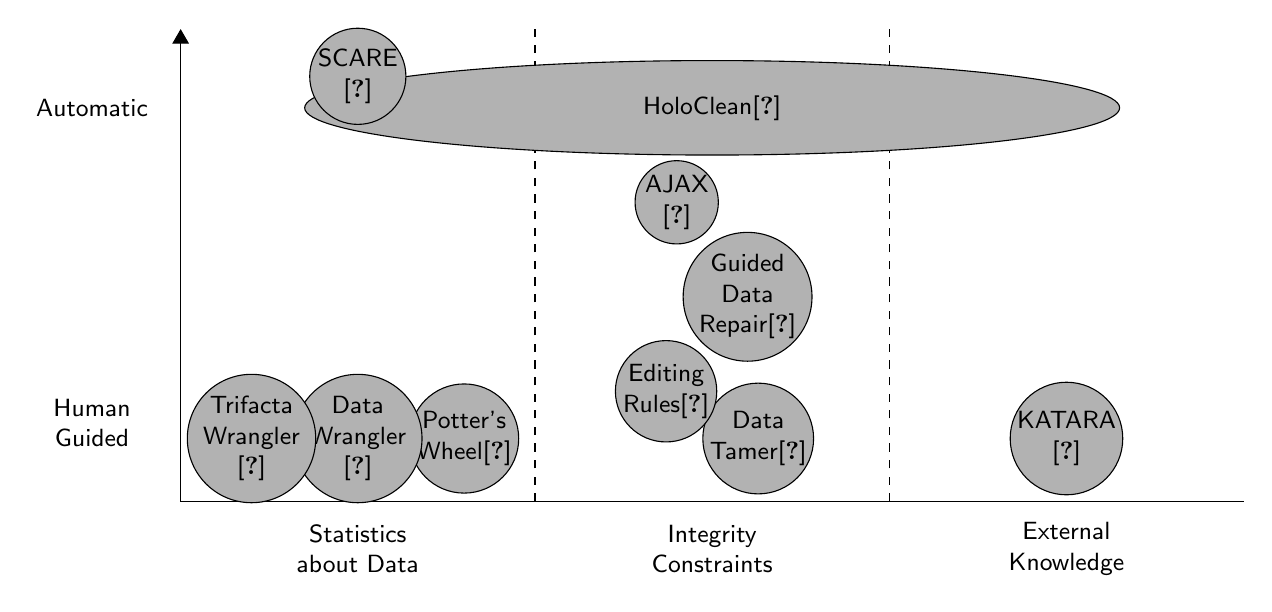
\begin{tikzpicture}[
    xscale=4.5, yscale=4,>=triangle 60,font=\sffamily,
    tool/.style={
      circle,
      draw=black,
      fill=black!30,
      inner sep=0pt,
      minimum size=25pt
    }
  ]
  \small  
  
  \begin{scope}
    \draw[black,] (-1.5,-0.25) -- (1.5,-0.25) ;
    \draw[black,->] (-1.5,-0.25) -- (-1.5,1.25) ;
    \draw[black,dashed] (-0.5,-0.25) -- (-0.5,1.25) ;
    \draw[black,dashed] (0.5,-0.25) -- (0.5,1.25) ;
    
    \draw[tool] (0,1) ellipse (1.15 and 0.15) node {\holoclean{}\cite{holoclean}};
    
    \node[tool, align=center] at (1,-0.05) {KATARA\\\cite{katara}};
    
    \node[tool, align=center] at (0.13,-0.05) {Data\\Tamer\cite{data_tamer}};
    \node[tool, align=center] at (-0.13,0.1) {Editing\\Rules\cite{editing_rules}};
    \node[tool, align=center] at (0.1,0.4) {Guided\\Data\\Repair\cite{gdr}};
    \node[tool, align=center] at (-0.1,0.7) {AJAX\\\cite{ajax}};
    
    \node[tool, align=center] at (-0.7,-0.05) {Potter's\\Wheel\cite{potters_wheel}};
    \node[tool, align=center] at (-1,-0.05) {Data\\Wrangler\\\cite{data_wrangler}};
    \node[tool, align=center] at (-1.3,-0.05) {Trifacta\\Wrangler\\\cite{trifacta_wrangler}};
    
    \node[tool, align=center] at (-1,1.1) {SCARE\\\cite{scare}};
    
    \node[align=center] at (-1.75,1) {Automatic};
    \node[align=center] at (-1.75,0) {Human\\Guided};
    
    \node[align=center] at (1,-0.4) {External\\Knowledge};
    \node[align=center] at (0,-0.4) {Integrity\\Constraints};
    \node[align=center] at (-1,-0.4) {Statistics\\about Data};
  
  \end{scope}
\end{tikzpicture}

\end{document}
    \caption{Data Repairing Tools in Context}
    \label{fig:tools}
  \end{figure*}

  \bigskip
  Most of the tools limit themselves to only one signal to perform data repairing, ignoring other information sources.
  Each type of signal is associated with a different action on the dataset and has its own downsides.
  Data repairs that use \glspl{ic} could introduce incorrect repairs, because they are relying on the \textit{minimality} principle and assume that most of the data values are clean.
  This is not necessarily the case and minimal repairs not always correspond to correct repairs~\cite{holoclean}.
  Repair algorithms relying on external information are dependent on the coverage of the external data source and can therefore perform poorly.
  Quantitative statistics heavily depend on the available information in the dataset itself.
  For small datasets and unfortunate situations this can drastically decrease repairing quality.
  
  \citeauthor{holoclean} therefore propose a holistic data repairing approach that includes all aforementioned signals into one framework: \holoclean{}~\cite{holoclean}.
  To tackle the problem that different signals could suggest conflicting repairs they convert all signals into features of a probabilistic model.
  Based on this combined view on the data and their inconsistencies they can then use statistical learning and probabilistic inference to suggest repairs for the dataset.
  
  \begin{itemize}
    \item \textbf{Paper Preview/Overview}
  \end{itemize}


\section{Background}\label{sec:background}
  In the following paragraphs we review the terminology used in the next sections.
  
  \subsection{Integrity Constraints}
  Users of the \holoclean{} framework can specify \glspl{ic} in form of denial constraints.
  They combine different types of integrity definitions.
  Functional Dependencies as well as conditional functional dependencies can be expressed as denial constraints~\cite{fd_to_dc}.
  A denial constraint states that all predicates of it cannot be true at the same time, otherwise, there is a consistency conflict.
  It is notated as $\forall t_i, t_j \in D: \neg(P_1 \wedge \dots \wedge P_K)$.
  Over all tuples $t \in D$ of a database instance $D$ not all predicates $P_k$ are allowed to be true.
  $P_k$ are defined as $v_1 \circ v_2$ or $v_1 \circ c$ with $v_1, v_2 \in \{t_i.A, t_j.A\}$, where $A$ denotes an attribute of the dataset $D$.
  The operator $\circ$ can be one of $\{=,<,>,\neq,\leq,\geq\}$~\cite{chu2013discoveringdc}.
  In this report we use functional dependencies of the form $t_i.A_1 \rightarrow t_j.A_2$ to express integrity constraints for readability reasons.
  They can easily converted to denial constraints~\cite{fd_to_dc}.
  
  \subsection{\deepdive{} and Factor Graphs}
  \holoclean{} relies on \deepdive{} to perform statistical learning and inference.
  It is a data management system developed at Stanford University, which allows scalable statistical inference on big unclean datasets~\cite{deepdive}.
  \holoclean{} uses \deepdive{} to create a factor graph over all input signals and data cells.
  The factor graph can be defined via a declarative language, called \ddlog{}.
  A collection of inference rules in DeepDive corresponds to a probabilistic model.
  Such inference rules are defined over a relation of random variables with weight annotations.
  We consider the following \ddlog{} rule as a template for the inference rules generated by the \holoclean{} framework:
  \begin{multline}
    Value?(t,a,d):-\\Relation(t,a,d), [\text{conditions}], weight=\text{w}
  \end{multline}
  $Value?(t,a,d)$ is the head of the rule and defines a random variable identified by $t$, $a$ and $d$.
  \holoclean{} uses $t$ to identify a tuple and $a$ to identify an attribute.
  $d$ corresponds to the value of cell $t.a$.
  The body of the rule consists of three parts:
  A number of other relations over the used variables (here only one: $Relation(t,a,d)$),
  conditions using the same operators like denial constraints enclosed in brackets and
  a weight annotation ($weight=\text{w}$).
  Grounding of those rules will generate the nodes and factors of the factor graph in \deepdive{}.
  

\section{The \holoclean{} Framework}\label{sec:framework}
  
  \subsection{Architecture Overview}
  In Figure~\ref{fig:architecture} ...
  
  \begin{figure}[hbt]
    \centering
    % !TeX root = holoclean.tex
% !TeX encoding = UTF-8
% !TeX spellcheck = en_US

% HoloClean Architecture
\begin{tikzpicture}[
    font=\sffamily,>=triangle 60,
    module/.style={
      draw=black,
      fill=white,
      align=center
    },
    io/.style={
      align=center
    },
    module arrow/.style={
      single arrow,
      %single arrow head extend=2.5mm,
      draw=black,
      %color=gray!20,
      shape border uses incircle,
      text height=1.5mm,
      text width=2.5mm,
      anchor=center
    }
  ]
  \small
  \newcommand{\vSep}{0.25cm}
  \newcommand{\hSep}{0.25cm}
  \newcommand{\fillColor}{black!30}
  
  % Inputs
  \node[io] (dataset) {Dataset};
  \node[io, right=\hSep of dataset] (ics) {Integrity\\Constraints};
  \node[io, right=\hSep of ics] (ext) {Matching\\Dependencies\\+ ext. Information};
  
  % HoloClean
  \path let
      \p1 = ($(ext.east)-(dataset.west)$),
      \p2 = (ext.east)
    in
      ($(dataset.west)+(\x1*.5,-1.5)$) node (text) {\textbf{HoloClean}};
  \node[module, below=\vSep*.5 of text] (module1) {1. Error Detection};
  \node[module, below=\vSep of module1] (module2) {2. Probabilistic\\Model Generation};
  \node[module, below=\vSep of module2] (module3) {3. Data Repairing};
  
  \begin{scope}[name=holocleanbg, on background layer]
    \node[draw=black, fill=\fillColor, fit=(text) (module3)] (holoclean) {};
  \end{scope}
  
  % Output
  \node[io, below left=6*\vSep and \hSep of module2.south] (confidence) {Confidence of\\Cell Assignments};
  \node[io, below right=6*\vSep and \hSep of module2.south] (cleaned) {Cleaned Dataset};
  
  % I/O connections
  \draw[black,->] (dataset.south) -- ($(holoclean.north)-(0.5,0)$);
  \draw[black,->] (ics.south) -- (holoclean.north);
  \draw[black,->] (ext.south) -- ($(holoclean.north)+(0.5,0)$);
  
  \draw[black,->] (holoclean.south) -- (confidence);
  \draw[black,->] (holoclean.south) -- (cleaned);
  
  % Detection
  \node[module arrow, left=\hSep*2 of module1.west, fill=\fillColor] (bigArrow) {};
  \node[module, left=\hSep of bigArrow,text=white] (detectors) {Detection\\Algorithms};
  \node[module, below left=1mm and 1mm of detectors.west, anchor=west] (detectors2) {Detection\\Algorithms};
\end{tikzpicture}
    \caption{\holoclean{} architecture overview}
    \label{fig:architecture}
  \end{figure}
    
  
  \subsection{Error Detection}

  \subsection{Generation of the probabilistic model}
  
  \subsection{Data Repairing}

\section{Performance of \holoclean{}}\label{sec:performance}

\section{Conclusion}\label{sec:conclusion}